\newcommand{\addImage}[2]{
  \begin{figure}[!htb]
    \begin{center}
      \includegraphics[width=5.5cm]{#1}
      \caption{#2} % description to image
      \renewcommand{\thefigure}{\thesubsection.\arabic{figure}}
    \end{center}
  \end{figure}
}

\newpage
\section{\Large{Architecture Design \& Implementation}}

\begin{enumerate}[label=\arabic*]
  \item {\large{Overall Architecture}}\\
    \begin{figure*}[!ht]
        \begin{center}
            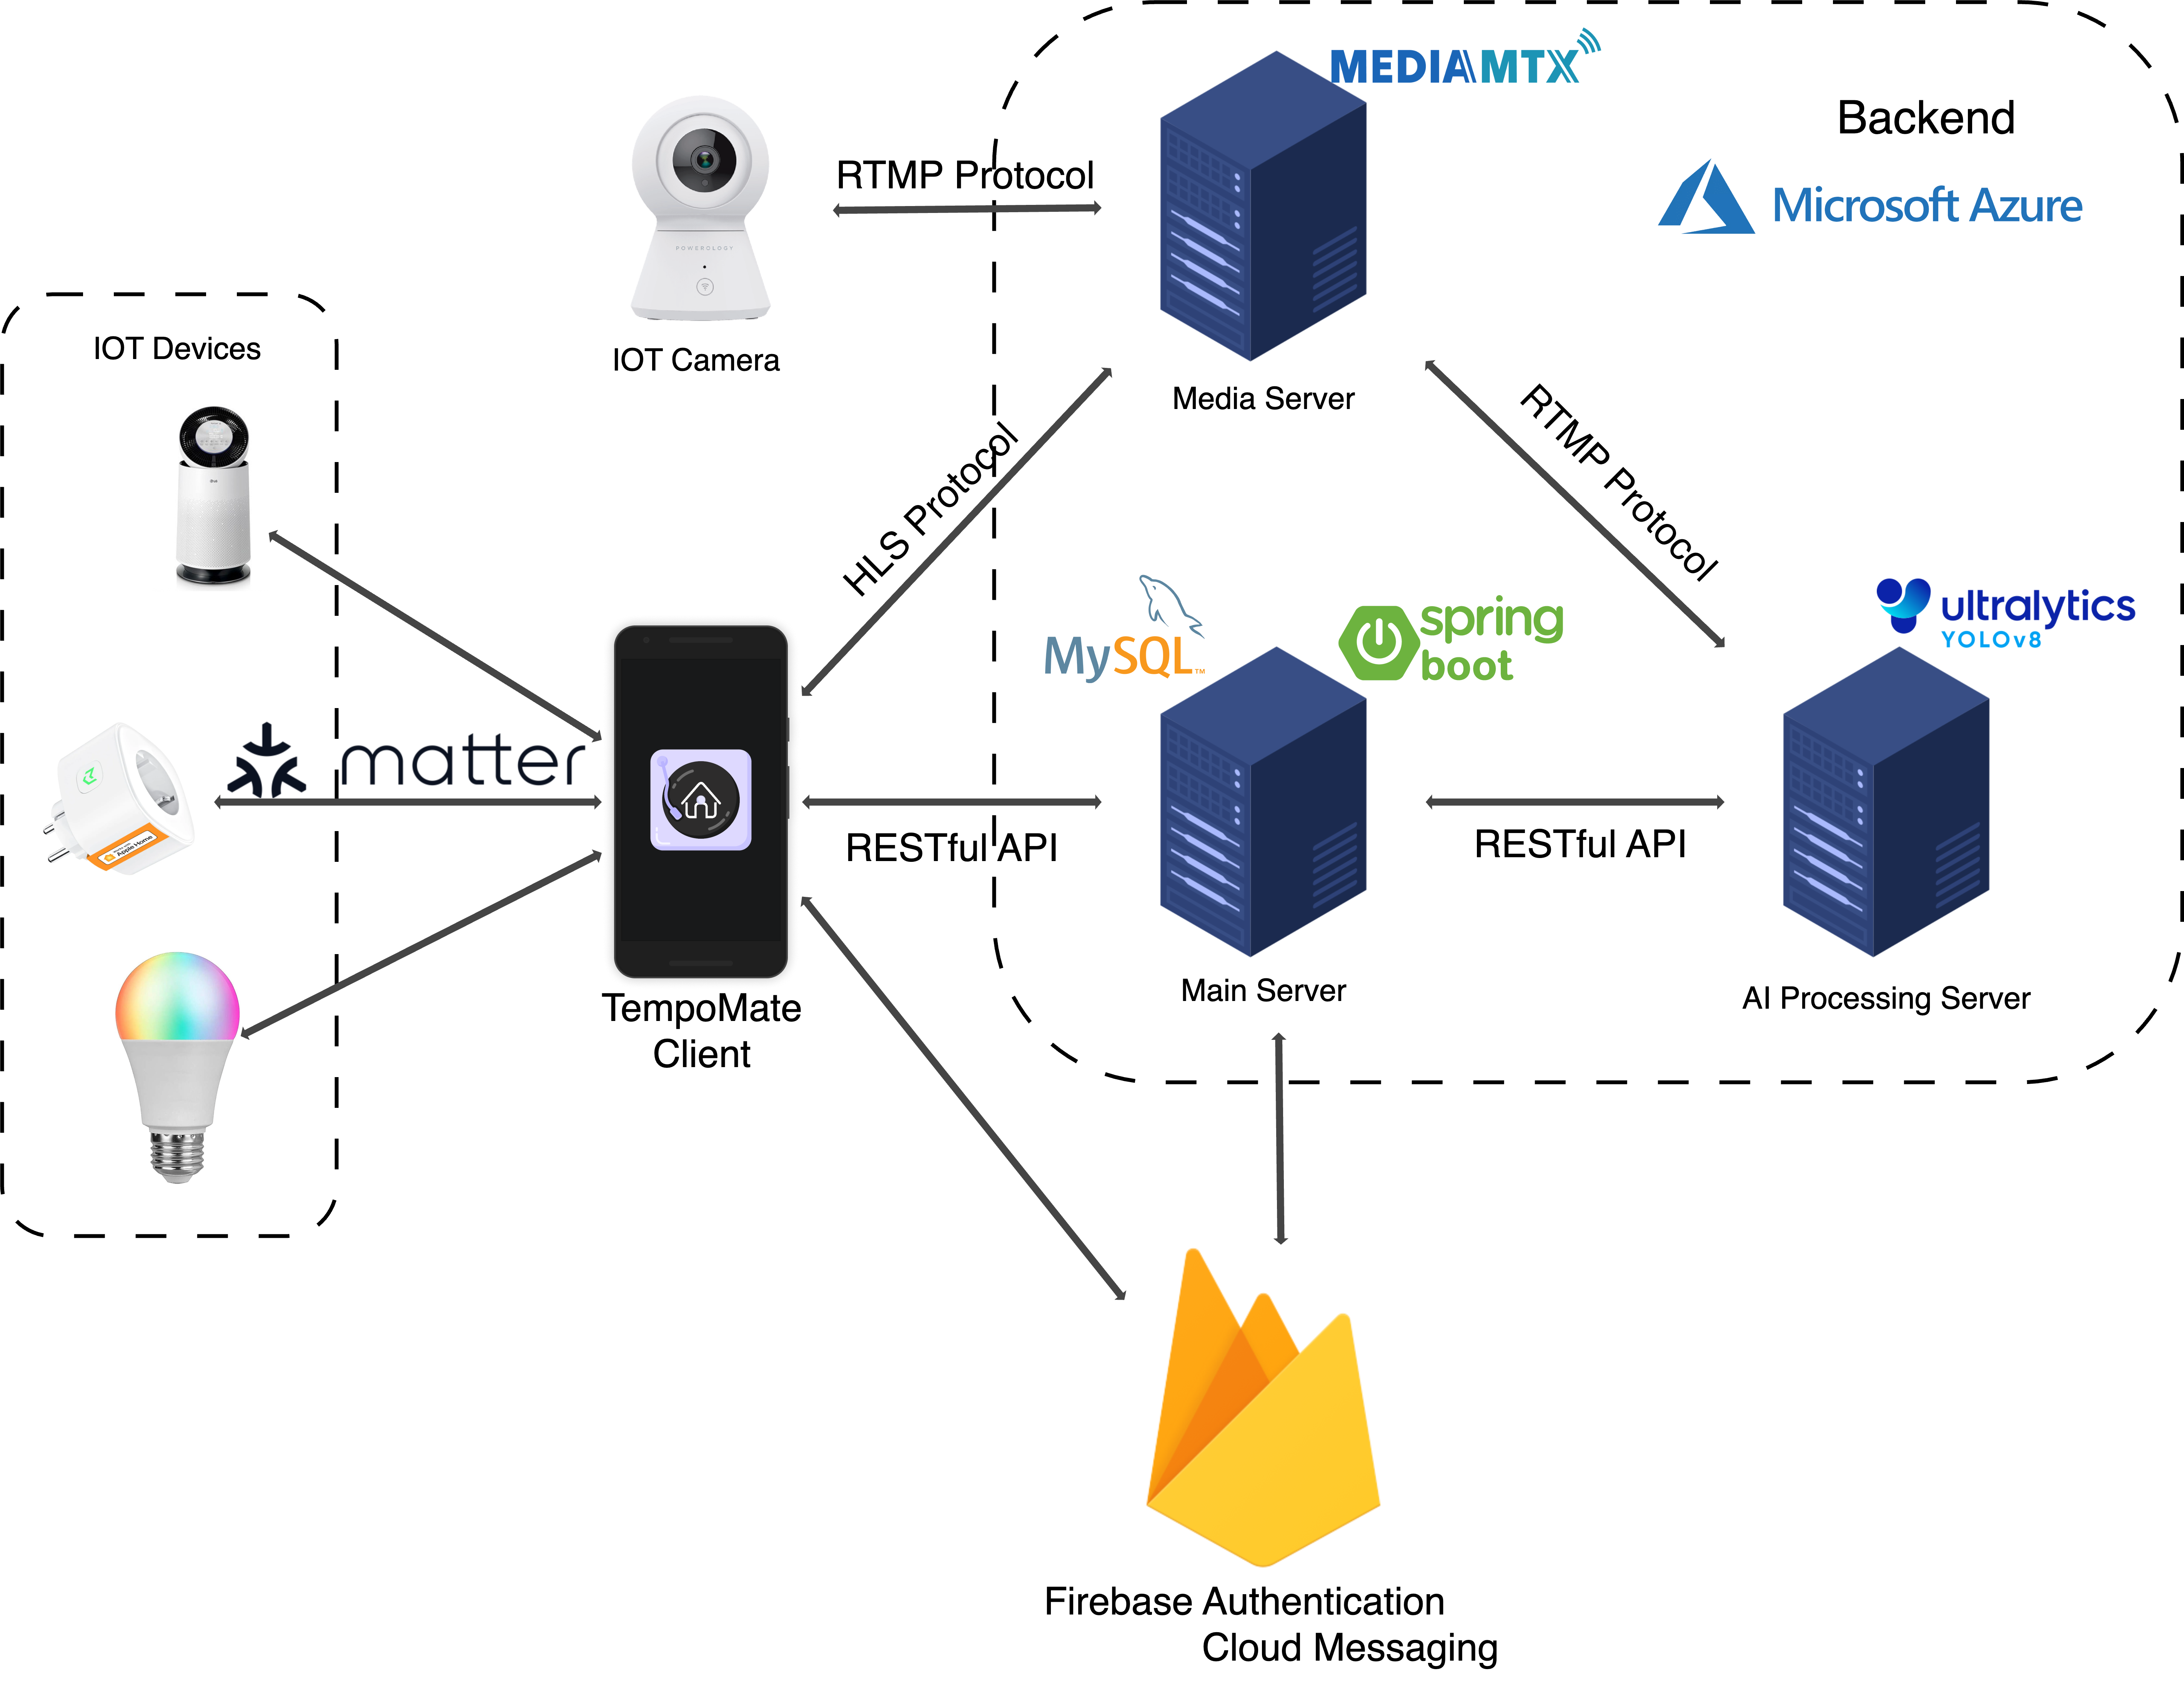
\includegraphics[width=14cm]{imgs/architecture.drawio.png}
            \caption{Architecture diagram} % description to image
            \renewcommand{\thefigure}{\thesubsection.\arabic{figure}}
        \end{center}
    \end{figure*}
    Our architecture consists of three main parts. IOT devices, an app frontend, and multiple backends.\\
    
    The IOT devices are connected to the TempoMate app frontend via the matter protocol. In general, the matter protocol can be remotely controlled externally through a separate hub, but in our project, we don't use a separate hub, but directly connect the smartphone and IOT devices to control them. The original plan was to connect to IOT cameras via matter, but the currently released version of the matter protocol does not support camera connections, so we used a different method.\\
     
    Our service uses cameras on both the frontend and backend, so we built a separate server that can connect to the IOT Camera and forward to the frontend and backend. With MEDIAMTX running on a separate server, the front and back end can always get a static IP. We use the RTMP protocol to send video from the IOT camera to the MEDIAMTX server, and the RTMP protocol to send video to the AI Processing server. The HLS protocol is used to receive video from the frontend. The AI Processing server receives the video and analyzes the frames to determine where the person is and what pose they are in, and the frontend actually watches the video to help determine where the person can be recognized.\\
    
    In order for the user to log in on the frontend, we use Firebase Authentication to get the user's information and authentication key, which we can then use to identify the user on the backend. Any saved routines, user names, or settings the user has changed on the frontend are passed to the main server via a RESTful API and stored. The saved information is retrieved the first time the user logs in and saved again whenever there are changes. \\
    
    To execute the routine through the Posture Trigger, the AI Processing server first gets the video from the Media server and analyzes the frame. If a person is detected after analyzing the frame, it gets the information about the triggers from the Main server and checks if there is a trigger corresponding to the detected information. If there is, it sends the data to the frontend to execute the routine associated with that trigger. This is where Firebase Cloud Messaging comes into play. Since the IP where the user is located is constantly changing and we can't see him in real time on the backend, we use a service provided by Google to send data directly to a specific smartphone. When the frontend receives this data, it runs the corresponding routine.\\
    
\newpage
  \item {\large{Directory Organization}}\\
        \begin{enumerate}[label=\alph*]
    \item Frontend\\

          \begin{description}
              \renewcommand{\makelabel}[1]{\textbf{\small #1}}

              \vspace{-0.2cm}
              \hrule
              \vspace{0.2cm}

              \item[/] \hfill \\
                    \small
                    - This folder contains the settings to build our project with graddle.\\\\
                    \footnotesize
                    gradle/libs.versions.toml  \\
                    gradle/wrapper/gradle-wrapper.jar  \\
                    gradle/wrapper/gradle-wrapper.properties  \\
                    gradlew  \\
                    build.gradle.kts  \\
                    settings.gradle.kts  \\
                    gradle.properties  \\
                    gradlew.bat  \\\\

                    \vspace{-0.2cm}
                    \hrule
                    \vspace{0.2cm}

              \item[/tempomate/] \hfill \\
                    \small
                    - This folder contains information about connecting to firebase and the dependencies used in our project.\\\\
                    \footnotesize
                    build.gradle.kts  \\
                    google-services.json  \\\\

                    \vspace{-0.2cm}
                    \hrule
                    \vspace{0.2cm}

              \item[/tempomate/third\_party/connectedhomeip/libs/] \hfill \\
                    \small
                    - This folder contains the libraries for using the Matter Protocol.\\\\
                    \footnotesize
                    AndroidPlatform.jar  \\
                    CHIPController.jar  \\
                    SetupPayloadParser.jar  \\
                    jniLibs/armeabi-v7a/libSetupPayloadParser.so  \\
                    jniLibs/armeabi-v7a/libCHIPController.so  \\
                    jniLibs/armeabi-v7a/libc++\_shared.so  \\
                    jniLibs/x86/libSetupPayloadParser.so  \\
                    jniLibs/x86/libCHIPController.so  \\
                    jniLibs/x86/libc++\_shared.so  \\
                    jniLibs/arm64-v8a/libSetupPayloadParser.so  \\
                    jniLibs/arm64-v8a/libCHIPController.so  \\
                    jniLibs/arm64-v8a/libc++\_shared.so  \\
                    jniLibs/x86\_64/libSetupPayloadParser.so  \\
                    jniLibs/x86\_64/libCHIPController.so  \\
                    jniLibs/x86\_64/libc++\_shared.so  \\\\

                    \vspace{-0.2cm}
                    \hrule
                    \vspace{0.2cm}

              \item[/tempomate/src/main/res/layout/] \hfill \\
                    \small
                    - This folder contains the fragments used by the application.\\\\
                    \footnotesize
                    fragment\_new\_device.xml  \\
                    fragment\_device\_sharing\_commissioning.xml  \\
                    fragment\_thread.xml  \\
                    fragment\_dummy\_device.xml  \\
                    fragment\_info.xml  \\
                    dropdown\_list\_item.xml  \\
                    fragment\_developer\_utilities\_settings.xml  \\
                    fragment\_admin.xml  \\
                    matter\_beacon\_view\_item.xml  \\
                    fragment\_home.xml  \\
                    fragment\_device.xml  \\
                    activity\_commissioning.xml  \\
                    fragment\_splash.xml  \\
                    fragment\_settings.xml  \\
                    fragment\_inspect.xml  \\
                    device\_view\_item.xml  \\
                    fragment\_codelab\_info\_checkbox.xml  \\
                    activity\_main.xml  \\
                    fragment\_commissionable.xml  \\\\

                    \vspace{-0.2cm}
                    \hrule
                    \vspace{0.2cm}

              \item[/tempomate/src/main/res/] \hfill \\
                    \small
                    - This folder contains resources such as themes, strings, pictures, icons, etc. that are used in our application.\\\\
                    \footnotesize
                    color/mtrl\_list\_item\_tint.xml  \\
                    values/colors.xml  \\
                    values/dimens.xml  \\
                    values/themes.xml  \\
                    values/strings.xml  \\
                    values/ids.xml  \\
                    navigation/navigation\_commissioning.xml  \\
                    navigation/navigation.xml  \\
                    ic\_playstore.png  \\
                    xml/settings\_developer\_utiltities\_screen.xml  \\
                    xml/settings\_preferences\_screen.xml  \\
                    menu/top\_app\_bar.xml  \\
                    menu/top\_app\_bar\_settings.xml  \\
                    menu/device\_topappbar\_menu.xml  \\
                    menu/home\_menu.xml  \\
                    ic\_playstore\_legacy.png  \\
                    ... \\\\

                    \vspace{-0.2cm}
                    \hrule
                    \vspace{0.2cm}

              \item[/tempomate/src/main/proto/] \hfill \\
                    \small
                    - This folder contains prototypes for some of the material types used in our application.\\\\
                    \footnotesize
                    devices.proto  \\
                    devices\_state.proto  \\
                    user\_prefs.proto  \\\\

                    \vspace{-0.2cm}
                    \hrule
                    \vspace{0.2cm}

              \item[/tempomate/src/main/] \hfill \\
                    \small
                    - This folder contains files that allow you to set permissions and details for our application.\\\\
                    \footnotesize
                    AndroidManifest.xml  \\\\

                    \vspace{-0.2cm}
                    \hrule
                    \vspace{0.2cm}

              \item[/.../setmp/tempomate/] \hfill \\
                    \small
                    - This folder is the entry point for activities and services that run at application startup.\\\\
                    \footnotesize
                    GHSAFM3pEcoApplication.kt  \\
                    MainActivity.kt  \\
                    Utils.kt  \\
                    IotScreen.kt  \\
                    FCMService.kt  \\\\

                    \vspace{-0.2cm}
                    \hrule
                    \vspace{0.2cm}

              \item[/.../setmp/tempomate/ui/] \hfill \\
                    \small
                    - This folder contains the files for what each page is made up of.\\\\
                    \footnotesize
                    Settings.kt  \\
                    Dashboard.kt  \\
                    DevicePage.kt  \\
                    Routines.kt  \\
                    ActionPage.kt  \\
                    IotViewModel.kt  \\
                    LogPage.kt  \\
                    AddActionSelectDevice.kt  \\
                    LoginPage.kt  \\
                    DeviceCard.kt  \\
                    RoutinePage.kt  \\
                    theme/Color.kt  \\
                    theme/Theme.kt  \\
                    theme/Type.kt  \\\\

                    \vspace{-0.2cm}
                    \hrule
                    \vspace{0.2cm}

              \item[/.../setmp/tempomate/auth/] \hfill \\
                    \small
                    - This folder contains class files to help with the sign in/up process.\\\\
                    \footnotesize
                    GoogleSignInHelper.kt  \\\\

                    \vspace{-0.2cm}
                    \hrule
                    \vspace{0.2cm}

              \item[/.../setmp/tempomate/chip/] \hfill \\
                    \small
                    - This folder contains classes for using the library for using the Matter protocol.\\\\
                    \footnotesize
                    ClustersHelper.kt  \\
                    MatterConstants.kt  \\
                    BaseCompletionListener.kt  \\
                    ChipClient.kt  \\
                    SubscriptionHelper.kt  \\\\

                    \vspace{-0.2cm}
                    \hrule
                    \vspace{0.2cm}

              \item[/.../setmp/tempomate/lifecycle/] \hfill \\
                    \small
                    - This folder contains files that cover the life cycle of the application.\\\\
                    \footnotesize
                    AppLifecycleObserver.kt  \\
                    HalfSheetSuppressionObserver.kt  \\
                    AppLifecycleObserverModule.kt  \\\\

                    \vspace{-0.2cm}
                    \hrule
                    \vspace{0.2cm}

              \item[/.../setmp/tempomate/screens/settings/] \hfill
                    \footnotesize
                    SettingsDeveloperUtilitiesNestedFragment.kt  \\
                    DeveloperUtilitiesViewModel.kt  \\
                    SettingsFragment.kt  \\
                    SettingsDeveloperUtilitiesFragment.kt  \\
                    SettingsNestedFragment.kt  \\\\

                    \vspace{-0.2cm}
                    \hrule
                    \vspace{0.2cm}

              \item[/.../setmp/tempomate/screens/home/] \hfill \\
                    \footnotesize
                    DevicesAdapter.kt  \\
                    HomeViewModel.kt  \\
                    HomeFragment.kt  \\
                    DeviceViewHolder.kt  \\\\

                    \vspace{-0.2cm}
                    \hrule
                    \vspace{0.2cm}

              \item[/.../setmp/tempomate/screens/inspect/] \hfill \\
                    \footnotesize
                    InspectViewModel.kt  \\
                    InspectFragment.kt  \\\\

                    \vspace{-0.2cm}
                    \hrule
                    \vspace{0.2cm}

              \item[/.../setmp/tempomate/screens/commissionable/] \hfill \\
                    \footnotesize
                    wifi/ModuleWifi.kt  \\
                    wifi/MatterBeaconProducerWifi.kt  \\
                    MatterBeaconInject.kt  \\
                    ble/ModuleBle.kt  \\
                    ble/MatterBeaconProducerBle.kt  \\
                    MatterBeaconAdapter.kt  \\
                    MatterBeacon.kt  \\
                    CommissionableViewModel.kt  \\
                    mdns/ModuleMdns.kt  \\
                    mdns/MatterBeaconProducerMdns.kt  \\
                    CommissionableFragment.kt  \\
                    MatterBeaconViewHolder.kt  \\
                    MatterBeaconProducer.kt  \\\\

                    \vspace{-0.2cm}
                    \hrule
                    \vspace{0.2cm}

              \item[/.../setmp/tempomate/screens/shared/] \hfill \\
                    \footnotesize
                    UserPreferencesViewModel.kt  \\
                    SelectedDeviceViewModel.kt  \\\\

                    \vspace{-0.2cm}
                    \hrule
                    \vspace{0.2cm}

              \item[/.../setmp/tempomate/screens/device/] \hfill \\
                    \footnotesize
                    DeviceFragment.kt  \\
                    DeviceViewModel.kt  \\\\

                    \vspace{-0.2cm}
                    \hrule
                    \vspace{0.2cm}

              \item[/.../setmp/tempomate/screens/thread/] \hfill \\
                    \footnotesize
                    ServiceDiscovery.kt  \\
                    OtbrHttpClient.kt  \\
                    ThreadViewModel.kt  \\
                    ThreadFragment.kt  \\\\

                    \vspace{-0.2cm}
                    \hrule
                    \vspace{0.2cm}

              \item[/.../setmp/tempomate/data/] \hfill \\
                    \small
                    - This folder contains the data classes, repositories, etc. that will be used in your application.\\\\
                    \footnotesize
                    UserDataRepository.kt  \\
                    UserPreferencesSerializer.kt  \\
                    DevicesStateSerializer.kt  \\
                    DevicesRepository.kt  \\
                    DevicesSerializer.kt  \\
                    UserPreferencesRepository.kt  \\
                    DevicesStateRepository.kt  \\
                    GsonInterfaceAdapter.kt  \\
                    Log.kt  \\
                    IotUiState.kt  \\
                    AppPreferenceDataStore.kt  \\
                    Action.kt  \\
                    Setting.kt  \\
                    Routine.kt  \\
                    Device.kt  \\\\\\

          \end{description}

    \item Backend\\

          \begin{description}
              \renewcommand{\makelabel}[1]{\textbf{\small #1}}

              \vspace{-0.2cm}
              \hrule
              \vspace{0.2cm}

              \item[/src/main/resources/static/] \hfill \\
                    \footnotesize
                    client.js \\
                    index.html \\
                    style.css \\\\
                    \vspace{-0.2cm}
                    \hrule
                    \vspace{0.2cm}

              \item[/src/main/resources/] \hfill \\
                    \footnotesize
                    application.properties \\\\
                    \vspace{-0.2cm}
                    \hrule
                    \vspace{0.2cm}

              \item[/src/main/java/com/tempomate/] \hfill \\
                    \footnotesize
                    SebackendApplication.java \\\\
                    \vspace{-0.2cm}
                    \hrule
                    \vspace{0.2cm}

              \item[/.../tempomate/mapper/] \hfill \\
                    \footnotesize
                    TriggerMapper.java \\
                    RoutineMapper.java \\
                    DeviceMapper.java \\
                    LogMapper.java \\
                    ActionMapper.java \\
                    UserMapper.java \\\\
                    \vspace{-0.2cm}
                    \hrule
                    \vspace{0.2cm}

              \item[/.../tempomate/controller/] \hfill \\
                    \footnotesize
                    DeviceController.java \\
                    TriggerController.java \\
                    LogController.java \\
                    ActionController.java \\
                    UserController.java \\
                    RoutineController.java \\\\
                    \vspace{-0.2cm}
                    \hrule
                    \vspace{0.2cm}

              \item[/.../tempomate/service/] \hfill \\
                    \footnotesize
                    DeviceService.java \\
                    UserService.java \\
                    RoutineService.java \\\\
                    \vspace{-0.2cm}
                    \hrule
                    \vspace{0.2cm}

              \item[/.../tempomate/service/impl/] \hfill \\
                    \footnotesize
                    DeviceServiceImpl.java \\
                    RoutineServiceImpl.java \\
                    UserServiceImpl.java \\\\
                    \vspace{-0.2cm}
                    \hrule
                    \vspace{0.2cm}

              \item[/.../tempomate/webrtc/] \hfill \\
                    \footnotesize
                    SocketHandler.java \\
                    WebSocketConfig.java \\
                    WebConfiguration.java \\\\
                    \vspace{-0.2cm}
                    \hrule
                    \vspace{0.2cm}

              \item[/.../tempomate/exception/] \hfill \\
                    \footnotesize
                    GlobalExceptionHandler.java \\\\

                    \vspace{-0.2cm}
                    \hrule
                    \vspace{0.2cm}

              \item[/.../tempomate/pojo/] \hfill \\
                    \footnotesize
                    Result.java \\\\
                    \vspace{-0.2cm}
                    \hrule
                    \vspace{0.2cm}

              \item[/.../tempomate/pojo/entity/] \hfill \\
                    \footnotesize
                    trigger/TriTime.java \\
                    trigger/TriAssistant.java \\
                    trigger/TriPosture.java \\
                    trigger/TriLocation.java \\
                    User.java \\
                    action/ActDevice.java \\
                    action/Action.java \\
                    action/ActTime.java \\
                    Device.java \\
                    Log.java \\
                    Routine.java \\\\\\

          \end{description}

    \item Computer vision\\
          \begin{description}
              \renewcommand{\makelabel}[1]{\textbf{\small #1}}

              \vspace{-0.2cm}
              \hrule
              \vspace{0.2cm}

              \item[/computer-vision/processing/] \hfill \\
                    \small
                    - This folder contains files about the cv backend.\\\\
                    \footnotesize
                    se-tmp-pk.json \\
                    model.pt \\
                    ThreadedCamera.py \\
                    Processor.py \\
                    FcmManager.py \\
                    main.py \\\\

                    \vspace{-0.2cm}
                    \hrule
                    \vspace{0.2cm}

              \item[/computer-vision/training/] \hfill \\
                    \small
                    - This folder contains files for training the model with our dataset.\\\\
                    \footnotesize
                    train.ipynb \\\\\\

          \end{description}
\end{enumerate}

        \newpage
  \item {\large{Architecture Implementation}}\\
        \begin{enumerate}[label=\alph*]
          \item Frontend\\
                \begin{enumerate}
                        \item Purpose \\
                              TempoMate's backend serves as the central nervous system, orchestrating seamless communication between users, frontend interfaces, and the intricate web of routines, triggers, and actions within the application. Its overarching purpose is to empower users to effortlessly manage their smart home environment, utilizing real-time video streaming via RTMP to detect user positions and postures, specifically when they are resting in bed. By understanding and interpreting these scenarios, the backend triggers predefined routines, seamlessly executing actions such as turning off room lights. Additionally, the backend administers essential user functionalities, including registration, login, logout, and nickname changes, ensuring a secure and personalized experience for each user. \\\\
                        \item Functionality \\
                              TempoMate offers an intuitive interface that empowers users to effortlessly harness the sophisticated capabilities orchestrated by the backend. The frontend serves as the user's gateway to a personalized and responsive smart home environment.\\

                              User Account Management:
                              The frontend streamlines the user account management process, providing a seamless experience for tasks such as registration, login, logout, and nickname changes. Through clear and user-friendly interfaces, individuals can easily establish and customize their profiles within the TempoMate ecosystem.\\

                              Routines Management:
                              Users have full control over defining their smart home environment through the frontend's management of routines. They can intuitively add, delete, and share routines, tailoring their automation preferences with simplicity. The frontend visually represents these routines, allowing users to grasp and modify their smart home orchestration effortlessly.\\

                              Action Customization:
                              The frontend facilitates the addition and deletion of actions, empowering users to specify precise responses to detected video scenarios. Through the frontend interface, users can fine-tune the behavior of their smart home, ensuring that it aligns precisely with their preferences and needs.\\

                              Trigger Activation:
                              Managing triggers becomes an accessible task through the frontend, enabling users to activate and expand smart home routines effectively. The frontend provides a clear representation of triggers, allowing users to understand and adjust the conditions that initiate specific actions within their smart home environment.\\

                              Real-time Video Streams:
                              The frontend seamlessly integrates real-time video streams captured via RTMP, providing users with live insights into their smart home environment. Through the frontend, users can monitor and interact with the captured video, enhancing their situational awareness and control.\\

                              In essence, the frontend of TempoMate not only simplifies user management but also empowers users to shape and interact with a smart home environment that is both adaptive and responsive, thanks to the sophisticated functionalities orchestrated by the backend. \\\\

                        \item Location of source code \\
                              : https://github.com/se-tmp/frontend \\\\

                        \item Class Component \\
                        \item[-] ActionPage.kt \\
                              The provided code includes several Jetpack Compose functions for building the user interface of an Android application. These functions handle different aspects of the app's functionality, such as selecting action types, choosing devices, and configuring actions for device control. The code demonstrates the use of Jetpack Compose features, creating a well-structured and maintainable codebase for managing the app's UI and user interactions.\\
                        \item[-] AddActionSelectDevice.kt \\
                              The AddActionSelectDevice composable class renders a grid of selectable devices retrieved from a DevicesRepository. Utilizing Jetpack Compose's LazyVerticalGrid, the devices are efficiently displayed in a two-column grid with appropriate spacing. Each device is represented by a DeviceCard with an associated icon and name. When a user selects a device by clicking on its card, the chosen device is stored in the IotViewModel, and the navigation is triggered to go back (onNavigateUp). This composable efficiently handles the presentation of selectable devices, enhancing the user experience for adding actions related to specific devices in the smart home environment\\
                        \item[-] Dashboard.kt \\
                              The Dashboard composable function renders a grid of devices, each represented by a DeviceCard, providing an overview of the smart home environment. The list of devices and their states is periodically updated by querying repositories (DevicesRepository and DevicesStateRepository). The devices are displayed in a two-column grid using LazyVerticalGrid, with appropriate spacing and padding. Each DeviceCard includes details such as the device name, icon, switch state, and online status. Users can interact with the cards by adjusting the device state or clicking on them to view more details. The composable uses coroutines to handle periodic updates of device information. This Dashboard composable serves as a central hub for users to monitor and control their smart home devices efficiently.\\
                        \item[-] DeviceCard.kt \\
                              The DeviceCard composable is a versatile component designed to represent various types of cards within a smart home application. It supports different card types (DeviceCardType), such as those for the dashboard, routines, and device selection. The card layout includes an icon, device name, and status information, with specific buttons or elements based on the card type. The card may feature an on/off switch (Switch) for the dashboard and routine cards, and it can handle adjustments with the provided onAdjust callback. Additionally, the card may display an "Offline" status for devices in the dashboard that are not currently online.\\
                        \item[-] DevicePage.kt \\
                              DevicePage serves as a comprehensive view for managing and interacting with a specific device, encompassing its status, actionable buttons, and a visual representation of the device. This composable enhances the user experience by providing a consolidated interface for device-related actions.\\
                        \item[-] IotViewModel.kt \\
                              The ViewModel initializes with user data repository, Gson for JSON serialization/deserialization, and loads initial data when created.\\\\
                              Loading Initial Data : Retrieves initially saved routines from the user data repository, parsing and updating the UI state accordingly.\\

                              Saving Routines : Asynchronously saves the provided list of routines to the user data repository in JSON format.\\

                              Setting User ID : Updates the UI state with the user ID.\\

                              Setting Device : Updates the UI state with the currently selected device.\\

                              Appending Action on Routine : Adds the current action to the actions list of the current routine in the UI state.\\

                              Appending Routine : Adds or modifies a routine in the UI state based on whether it already exists.\\

                              Deleting Action on Routine by Index : Removes an action from the actions list of the current routine based on the provided index.\\

                              Setting Current Action : Updates the UI state with the current action.\\

                              Setting Actions : Updates the UI state with a list of actions.\\

                              Setting Trigger Type of Current Routine : Updates the UI state with the trigger type of the current routine.\\

                              Setting Trigger of Current Routine : Updates the UI state with the trigger of the current routine.\\

                              Setting Triggers : Updates the UI state with a list of triggers.\\

                              Setting Routines : Updates the UI state with a list of routines.\\

                              Setting Current Routine : Updates the UI state with the current routine.\\
                        \item[-] LoginPage.kt \\
                              The provided code comprises three Jetpack Compose functions for user authentication in an IoT application. LoginPage displays a login page, allowing users to sign in with email/password or Google. SignIn handles email/password authentication, while SignUp manages user registration. These functions utilize FirebaseAuth for authentication and seamlessly navigate to the Devices screen upon successful login or signup, enhancing the overall user authentication flow.\\
                        \item[-] RoutinePage.kt \\
                              The provided code includes Jetpack Compose functions for creating various UI components related to an IoT application. TitleBar, TitleButtons, TriggerTypes, Trigger, AddActionButton, Action-ControlDevice, Action, Actions, RoutinePage, PointerCircle, and ResizableRectangle contribute to building the user interface for managing routines and actions. These components cover aspects such as displaying routine titles, handling triggers, showing action lists, and providing interactive elements for creating and editing routines.\\
                        \item[-] Routines.kt \\
                              Routines is a Composable function that uses Jetpack Compose to display a grid of routine cards. It takes an IotViewModel as a parameter to access the UI state, a function onClickCard to be executed when a routine card is clicked, and an optional modifier for styling. The routine data is collected from the UI state using viewModel.uiState.collectAsState().value.routines.\\

                              The grid is implemented using LazyVerticalGrid with fixed columns, and each routine is represented by a DeviceCard composable. The DeviceCard includes information such as the routine's name, icon, and on/off status. When a routine card is clicked, it updates the current routine in the view model and triggers the onClickCard function.\\
                        \item[-] Settings.kt \\
                              Settings is a Composable function that represents a screen displaying user settings, including a title bar, notification settings, backup and restore options, version information, and a delete all settings option. It utilizes Jetpack Compose for UI development and Firebase Authentication (auth: FirebaseAuth) for handling user authentication. The screen layout is organized using various Compose components such as Column, Row, Text, Icon, Switch, and Button.\\
                        \item[-] LotScreen.kt \\
                              The App Composable function represents the main structure of your IoT application. It uses Jetpack Compose for UI development and is composed of various screens corresponding to different IotScreen enum values. The app includes features such as user authentication, a dashboard displaying devices, routines management, logs, settings, and various actions. The App Composable orchestrates the navigation flow, state management, and UI structure of your IoT application, providing a cohesive user experience across different screens.\\
                        \item[-] FCMService.kt \\
                              The FCMService class extends FirebaseMessagingService and overrides the onMessageReceived method to handle incoming FCM messages. When a message is received, it logs the message details using Timber and extracts a target value from the message data. It then initiates a routine using the startRoutine method of the IotViewModel associated with the FCMManager singleton.
                              The FCMManager class is a singleton responsible for managing the FCM instance. It holds a reference to an IotViewModel and ensures a single instance of itself is created using the Singleton pattern. The context is initialized when the instance is created.\\
                        \item[-] Action.kt\\
                              ActionType: An enumeration defining the types of actions with associated titles, icons, and numerical identifiers.
                              Action: An interface specifying properties for actions.
                              ActDevice: A data class representing details about a device-related action. It implements the Action interface, inheriting basic properties for actions.\\
                        \item[-] AppPreferenceDataStore.kt\\
                              code defines a custom PreferenceDataStore for managing application settings data. This custom data store interacts with a UserPreferencesRepository, which appears to be a Proto DataStore managing user preferences. The AppPreferenceDataStore class handles storing and retrieving settings, converting between string and boolean values based on certain keys, and updating the underlying data repository accordingly.
                              The use of coroutines and asynchronous operations demonstrates an approach to managing data interactions without blocking the main thread. The code also utilizes Timber for logging.\\
                        \item[-] Device.kt\\
                              DeviceType: An enumeration defining different types of devices, including an unknown type and three specific types (SLIDER-BULB, SWITCH-BULB, SWITCH).
                              Device: A data class representing device information, including the device's ID, name, type (using the DeviceType enum), switch status, and text information.
                              The code is relevant to a device table, and the data class makes it convenient to manipulate and utilize device details within the application.\\
                        \item[-] DevicesRepository.kt\\
                              DevicesRepository responsible for managing and persisting a set of devices using a DataStore.
                              The DevicesRepository is a singleton repository that interacts with a DataStore to manage and persist a collection of devices in the homesampleapp fabric. It provides methods to add, update, remove, and retrieve devices, as well as to clear all data. The repository uses coroutines and provides a Flow for observing changes in the stored devices.
                              The incrementAndReturnLastDeviceId method increments the last device ID and updates the DataStore. The addDevice method adds a new device, updateDevice updates an existing device, removeDevice removes a device, and getDevice retrieves a specific device by ID. Additionally, there are methods to update the device type, get the last device ID, and retrieve all devices.\\
                        \item[-] DevicesSerializer.kt\\
                              The DevicesSerializer object implements the Serializer interface for the Devices data type. It specifies how to convert instances of Devices to and from bytes for storage and retrieval. In case of a protocol buffer parsing exception, a CorruptionException is thrown to handle potential data corruption.

                              The extension property devicesDataStore is created as an extension property on the Context class. It provides a convenient way to obtain a DataStore<Devices> instance with the specified file name ("devices-store.proto") and the custom DevicesSerializer. This extension property simplifies the creation of the DataStore for managing instances of the Devices class.\\
                        \item[-] DevicesStateRepository.kt\\
                              The DevicesStateRepository is a singleton repository that interacts with a DataStore to manage and persist the dynamic state of devices in the homesampleapp fabric. It provides methods to add, update, and retrieve device states, as well as to clear all data. The repository uses coroutines and provides a Flow for observing changes in the stored devices' dynamic states.

                              The repository maintains a LiveData (lastUpdatedDeviceState) representing the latest device state update. This LiveData is updated whenever a new device state is added or an existing one is updated.

                              The addDeviceState method adds a new device state, and the updateDeviceState method updates an existing device state. The repository ensures that the LiveData reflecting the last updated device state is always kept current.

                              The getAllDevicesState method retrieves the entire dynamic state of devices, and the clearAllData method clears all stored data.\\
                        \item[-] DevicesStateSerializer.kt\\
                              The DevicesStateSerializer object implements the Serializer interface for the DevicesState data type. It defines how to convert instances of DevicesState to and from bytes for storage and retrieval. If there's an issue with parsing the protocol buffer during deserialization, a CorruptionException is thrown to handle potential data corruption.

                              The extension property devicesStateDataStore is created as an extension property on the Context class. This property provides a convenient way to obtain a DataStore<DevicesState> instance with the specified file name ("devices-state-store.proto") and the custom DevicesStateSerializer. This extension property simplifies the creation of the DataStore for managing instances of the DevicesState class.\\
                        \item[-] GsonInterfaceAdapter.kt\\
                              The GsonInterfaceAdapter class implements both the JsonDeserializer and JsonSerializer interfaces for handling the serialization and deserialization of interface types. It utilizes Gson's functionality to convert JSON elements to Java objects and vice versa.

                              The deserialize method is responsible for deserializing a JSON element into an object of the specified interface type. It extracts the class name and data from the JSON element, resolves the class, and then uses Gson's context to deserialize the data into an object of the resolved class.

                              The serialize method is responsible for serializing an object of an interface type into a JSON element. It creates a JSON object, adds the class name and serialized data to it, and returns the resulting JSON element.

                              The companion object defines constants for the keys used in the JSON representation (CLASSNAME for the class name and DATA for the data).\\
                        \item[-] IotUiState.kt\\
                              The IotUiState data class encapsulates various properties that collectively represent the current state of the IoT user interface.\\

                              currentRoutine: The currently selected routine.\\
                              routines: A list of available routines.\\
                              actions: A list of actions associated with the IoT application.\\
                              triggers: A list of triggers for routines.\\
                              device: Information about a specific device.\\
                              currentAction: The currently selected action.\\
                              userId: The user ID associated with the state.\\
                        \item[-] Routine.kt\\
                              The TriggerType enum represents different types of triggers, such as Location, Posture, Assistant, Time, and Sensor. Each type is associated with a numeric identifier (num) and an ImageVector icon.

                              The Routine data class represents an IoT routine, including properties such as id, user-id, name, isOn (indicating whether the routine is turned on), trigger-type (the type of trigger), trigger-id, and a list of associated actions (actions). It also contains a reference to the specific trigger (trigger).

                              The PostureEnum enum represents different posture modes (Sit, Stand, Lie) and is used in the TriPosture class.

                              The TriPosture data class implements the Trigger interface, representing a posture trigger. It includes properties like id, type, detectPosture (posture mode), and coordinates for the trigger area.

                              The TriTime data class implements the Trigger interface, representing a time-based trigger. It includes properties like id, type, and time (representing the trigger time).\\
                        \item[-] UserDataRepository.kt\\
                              The UserDataRepository class provides functionality to save and retrieve user routines using a DataStore<Preferences> instance.\\
                        \item[-] UserPreferencesRepository.kt\\
                              This repository provides methods to update and retrieve user preferences using a DataStore instance.

                              userPreferencesDataStore: A DataStore instance for managing user preferences.\\

                              userPreferencesFlow: A Flow property that emits user preferences. It catches exceptions during data reading, emitting the default instance if an IOException occurs.\\
                              userPreferencesLiveData: Converts userPreferencesFlow to LiveData for use in Android's LiveData-based components.\\

                              updateHideCodelabInfo(hide: Boolean): Updates the preference for hiding codelab information.\\
                              updateHideOfflineDevices(hide: Boolean): Updates the preference for hiding offline devices.\\
                              shouldShowHalfsheetNotification(): Retrieves whether to show the half-sheet notification.\\
                              updateShowHalfsheetNotification(show: Boolean): Updates the preference for showing the half-sheet notification.\\
                              isHideCodelabInfo(): Retrieves whether codelab information should be hidden.\\
                              getData(): Retrieves the current user preferences.\\
                        \item[-] UserPreferencesSerializer.kt\\
                              UserPreferencesDataStore: A DataStore instance for managing user preferences.
                              It uses the user-prefs-store.proto file as the serialized data storage format.
                              The serialization and deserialization logic is implemented in the UserPreferencesSerializer object.\\
                              defaultValue: The default value for the UserPreferences if deserialization fails.\\
                              readFrom(input: InputStream): Deserializes the protobuf data from the input stream.\\
                              writeTo(t: UserPreferences, output: OutputStream): Serializes the UserPreferences to the output stream.\\
                        \item[-] GoogleSignInHelper.kt\\
                              GoogleSignInHelper class encapsulates the logic for initiating and handling Google Sign-In operations. It integrates with Firebase Authentication and utilizes the Identity API for a streamlined sign-in experience. The class is designed to work with Flows, making it suitable for use in coroutine-based Android applications.\\

                    \end{enumerate}

                \newpage
          \item Backend\\
                \begin{enumerate}
    \item Purpose \\
          TempoMate's backend serves as the central nervous system, orchestrating seamless communication between users, frontend interfaces, and the intricate web of routines, triggers, and actions within the application. Its overarching purpose is to empower users to effortlessly manage their smart home environment, utilizing real-time video streaming via RTMP to detect user positions and postures, specifically when they are resting in bed. By understanding and interpreting these scenarios, the backend triggers predefined routines, seamlessly executing actions such as turning off room lights. Additionally, the backend administers essential user functionalities, including registration, login, logout, and nickname changes, ensuring a secure and personalized experience for each user. \\\\

    \item Functionality \\
          The backend of TempoMate enhances user experience and enables various functionalities for smart home automation. It efficiently handles user account management tasks, including user registration, authentication (login/logout), and user nickname changes. The core of the app lies in its capability to manage routines, allowing users to define their smart home environment easily through features such as adding, deleting, and sharing routines. Similarly, the backend manages the addition and deletion of actions, enabling users to define specific responses to detected video scenarios. Additionally, the backend facilitates the effective activation of smart home routines by managing the addition and expansion of triggers. Lastly, the backend seamlessly processes real-time video streams captured via RTMP, forwarding them to the frontend and AI components to perform their respective functions. In summary, the multifaceted functionalities of the backend not only ensure a robust user management system but also establish a responsive and adaptive smart home environment based on AI and routines. \\\\

    \item Location of source code \\
          : www.github.com/se-tmp/backend \\\\

    \item Database Implementation\\
          % \begin{enumerate}[label=\alph*]
            \begin{figure*}[!htb]
                \begin{center}
                    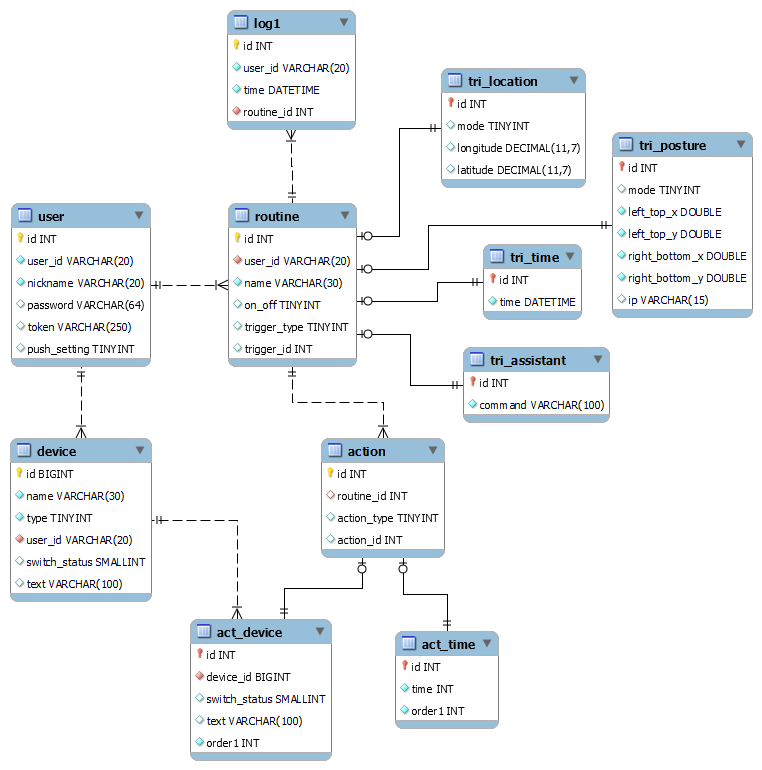
\includegraphics[width=12cm]{imgs/architecture_design_and_implementation/database-erd.png}
                    \caption{Database ERD} 
                    \renewcommand{\thefigure}{\thesubsection.\arabic{figure}}
                \end{center}
            \end{figure*}
          % \addImage{
          %     imgs/architecture_design_and_implementation/database-erd.png
          % }{
          %     Database Diagram
          % }
          This is the database that our architecture is currently using. This database consists of 11 tables. By using the structure of these tables, the data generated by the project can be stored.\\
          \begin{enumerate}
              \item user
                    \begin{itemize}
                        \item Used to store registered user information.
                        \item Primary Key: id (auto-increment, unique identifier in the user table), used for indexing data in the table.
                        \item user\_id: varchar(30), a unique identifier for the user. Used to differentiate between different users in the system.
                        \item nickname: varchar(30), the user's nickname. Displayed on the user interface for personalizing the user experience.
                        \item password: varchar(64), the user's password used for authentication during login. Should be stored encrypted in MD5 format to ensure data security.
                        \item token: varchar(250), the user's token used for authentication and access control, ensuring the security of sensitive operations.
                        \item push\_setting: tinyint, default value 1, push notification settings; 0 indicates disabled, 1 indicates enabled. Controls the status of push notifications in the app.\\
                    \end{itemize}

              \item device
                    \begin{itemize}
                        \item Used to store information about devices connected by users.
                        \item Primary Key: id (auto-increment, unique identifier in the device table), stored in bigint format to accommodate larger device IDs.
                        \item name: varchar(30), the name of the device used for identification and description, allowing users to customize the device name displayed in the app.
                        \item type: tinyint, device type, used for categorizing and distinguishing different types of devices. For example, when it is 1, it represents a sliding light bulb, 2 is a switch light bulb, 3 is a general switch, and so on. Different control components are displayed in the app based on the device type.
                        \item user\_id: varchar(20), linked to the user\_id in the user table, used to identify the owner of the device, ensuring that the device is associated with a specific user.
                        \item switch\_status: smallint, default value 0, represents the on/off status of the device, with values ranging from 0 to 100, indicating the current state of the device.
                        \item text: varchar(100), the device's IP address or command, used for communication and control of the device or for storing other necessary information.\\
                    \end{itemize}

              \item routine
                    \begin{itemize}
                        \item Used to store various routine information saved by users.
                        \item Primary Key: id (auto-increment, unique identifier in the routine table), used for indexing data in the table.
                        \item user\_id: varchar(20), linked to the user\_id in the user table, identifying the owner of the routine, ensuring that the routine is associated with a specific user.
                        \item name: varchar(30), the name of the routine, used to save the user-set routine name.
                        \item on\_off: tinyint, default value 0, the on/off status of the routine, where 0 indicates off and 1 indicates on, controlling the activation status of the routine.
                        \item trigger\_type: tinyint, trigger type, used to indicate which type of trigger will activate this routine. For example, 1 represents location-based triggering, and 2 represents posture recognition triggering.
                        \item trigger\_id: int, linked to the IDs in various trigger tables, used to establish the association between the routine and trigger conditions.\\
                    \end{itemize}

              \item tri\_location
                    \begin{itemize}
                        \item This table is used to store location-based trigger information.
                        \item Primary Key: id (auto-increment, unique identifier in the location trigger table), used for indexing data in the table.
                        \item mode: tinyint, default value 0, mode where 0 represents triggering on entry, and 1 represents triggering on exit. Determines the type of location trigger.
                        \item longitude: decimal(11, 7), longitude representing the coordinates of the location. Used to define the geographic location for location-based triggering.
                        \item latitude: decimal(11, 7), latitude representing the coordinates of the location. Used to define the geographic location for location-based triggering.\\
                    \end{itemize}

              \item tri\_posture
                    \begin{itemize}
                        \item Used to store the screen range to be recognized by the camera.
                        \item Primary Key: id (auto-increment, unique identifier in the posture trigger table), used for indexing data in the table.
                        \item mode: tinyint, default value 0, mode where 0 represents sitting posture triggering, 1 represents standing posture triggering, and 2 represents lying posture triggering. Used to determine the type of posture trigger.
                        \item left\_top\_x: double, the X coordinate of the top-left corner used to define the x-axis of the top-left corner of the posture trigger area. Determines the triggering area for posture recognition.
                        \item left\_top\_y: double, the Y coordinate of the top-left corner used to define the y-axis of the top-left corner of the posture trigger area. Determines the triggering area for posture recognition.
                        \item right\_bottom\_x: double, the X coordinate of the bottom-right corner used to define the x-axis of the bottom-right corner of the posture trigger area. Determines the triggering area for posture recognition.
                        \item right\_bottom\_y: double, the Y coordinate of the bottom-right corner used to define the x-axis of the bottom-right corner of the posture trigger area. Determines the triggering area for posture recognition.
                        \item ip: varchar(15), can be used for the camera's IP address if needed.\\
                    \end{itemize}

              \item tri\_assistant
                    \begin{itemize}
                        \item Used to store characters or sentences that need to be recognized.
                        \item Primary Key: id (auto-increment, unique identifier in the assistant trigger table), used for indexing data in the table.
                        \item command: varchar(100), can be used to store an IP address or command for voice recognition.\\
                    \end{itemize}

              \item tri\_time
                    \begin{itemize}
                        \item Used to store the time required for time triggers.
                        \item Primary Key: id (auto-increment, unique identifier in the time trigger table).
                        \item time: datetime, stores the trigger time, used to specify when operations related to this time should be triggered.\\
                    \end{itemize}

              \item action
                    \begin{itemize}
                        \item Serves as the main table for actions, allowing data related to actions to be retrieved based on their types and IDs.
                        \item Primary Key: id (auto-increment, unique identifier in the action table), used for indexing data in the table.
                        \item routine\_id: int, linked to the ID in the routine table, indicating the routine associated with this action. Establishes the association between actions and routines.
                        \item action\_type: tinyint, action type, where 1 represents device actions and 2 represents time-delayed time actions. Used to determine the type of action.
                        \item action\_id: int, linked to the ID in the corresponding action type table. Using the action type data and action ID, specific information about the action can be retrieved.\\
                    \end{itemize}

              \item act\_device
                    \begin{itemize}
                        \item Used to store the state to which devices should be changed after action triggers.
                        \item Primary Key: id (auto-increment, unique identifier in the device action table), used for indexing data in the table.
                        \item device\_id: bigint, linked to the ID in the device table, indicating the device to be controlled. Establishes the association between actions and devices.
                        \item switch\_status: smallint, default value 0, represents the switch status to be modified by the action, with values ranging from 0 to 100.
                        \item text: varchar(100), used to store the device's IP address or command, specifying the specific operation of the device action.
                        \item order1: int, indicates the order in which the action should be executed. Used to determine the execution order when multiple actions are present.\\
                    \end{itemize}

              \item act\_time
                    \begin{itemize}
                        \item Stores the specific time for delayed triggers.
                        \item Primary Key: id (auto-increment, unique identifier in the time action table), used for indexing data in the table.
                        \item time: int, time in seconds, indicating the time delay for executing the action. Used to specify the triggering time for time actions.
                        \item order1: int, indicates the order in which the action should be executed. Used to determine the execution order when multiple actions are present.\\
                    \end{itemize}

              \item log1
                    \begin{itemize}
                        \item Stores log trigger records.
                        \item Primary Key: id (auto-increment, unique identifier in the log table), used for indexing data in the table.
                        \item user\_id: varchar(20), linked to the user\_id in the user table, indicating the user to whom the log belongs. Ensures that the log is associated with a specific user.
                        \item time: datetime, records the time the log was generated. Used to track the time of events.
                        \item routine\_id: int, linked to the ID in the routine table, indicating the routine associated with the log. Used to indicate which routine triggered this log record.\\
                    \end{itemize}

          \end{enumerate}
    \item Class Component \\
    \item[-] pom.xml: This file is associated with the Maven build management tool commonly used in Java projects. It contains project configuration information and is written in XML format. It is used to define project settings, dependencies, plugins, and other build-related information.\\
    \item[-] src/main/resources/application.properties : This configuration file defines settings for a Spring Boot application, specifying the context path as "/api" and providing connection details for a MySQL database.\\
    \item[-] src/main/java/com.tempomate/controller: This is the folder that contains controllers which handle user input and return the results to the user. \\
    \item[-] ActionController: This class handles API operations related to actions using POST, GET, and DELETE mappings. The "/actDevice\_add" and "/actTime\_add" endpoints use POST requests to respectively add device actions and time delay actions. The "/get\_all\_action/\{userId\}" endpoint retrieves all actions stored in the database using a GET request, where \{userId\} is the user identifier. The "/delete/\{id\}" endpoint deletes the action corresponding to the provided ID from the database using a DELETE request.\\
    \item[-] DeviceController: This class handles various mappings related to devices, including POST, DELETE, GET, and PUT. The "/add" endpoint uses POST to add a device to the database. The "/delete/\{id\}" endpoint, using DELETE, removes the device with the specified ID from the database. The "/get\_all\_device/\{userId\}" endpoint, with GET, returns all devices associated with the given user ID. The "/rename\_device" endpoint, using PUT and receiving a new device name in the request body, updates the device name. Lastly, the "/change\_status" endpoint, through PUT, receives a request to change the device's switch within the range of 0 to 100. \\
    \item[-] LogController: This class handles logging, and the "/user/\{userId\}" endpoint, through a GET mapping, returns a list of all logs for the user corresponding to the user ID in the endpoint. \\
    \item[-] RoutineController: This class handles various mappings related to routines, encompassing POST, DELETE, GET, and PUT methods. The "/add" endpoint is used to create a new routine using a POST request. The "/delete/\{id\}" endpoint, through a DELETE mapping, processes the deletion of the routine associated with the provided ID. The "/get\_all\_routine/\{userId\}" endpoint, utilizing the GET method, returns a list of all routines associated with the specified `\{userId\}` value. The "/rename\_routine" endpoint, receiving a request for a new routine name, updates the routine's name using a PUT request. Finally, the "/change\_status" endpoint, taking the routine's ID and on/off status in the request body, updates the routine's on/off status using a PUT request. \\
    \item[-] TriggerController: This class uses POST mappings to add triggers and GET mappings to retrieve them. The endpoints "/loc\_add," "/pos\_add," "/assi\_add," and "/time\_add" are used to respectively add location triggers, posture triggers, assistant triggers, and time triggers through POST requests. The "/get" endpoint receives triggerType and triggerId in the request and returns the corresponding trigger using a POST mapping. Additionally, conditional statements are used to fetch different triggers based on the trigger type of the routine. For each trigger type, it retrieves the appropriate trigger (TriLocation, TriPosture, TriAssistant, TriTime) from the database. \\
    \item[-] UserController: This class handles user-related information using POST and PUT mappings. The "/signup" endpoint deals with user registration using a POST request. The "/login" endpoint is a POST API that receives the user's ID and password in the request for performing login. The "/rename-nickname" endpoint updates the user's nickname by receiving a new nickname through a PUT request. The "/push\_setting" endpoint manages the user's push notification status using a PUT request.\\
    \item[-] src/main/java/com.tempomate/exception/ \par GlobalExceptionHandler: This code defines a global exception handler in a Spring Boot application.\\
    \item[-] src/main/java/com.tempomate/mapper : This is the folder that is employed to define and execute SQL queries for interacting with a database. \\
    \item[-] ActionMapper: This interface interacts with the database to provide functionality related to actions. The `addAction`, `addActDevice`, and `addActTime` methods are responsible for adding action, device action, and time delay action, respectively, to the database. The `getActDevice` and `getActTime` methods retrieve device actions and time delay actions associated with a user and routine. Lastly, the `deleteAction` method removes all action data from the database. \\
    \item[-] DeviceMapper: This interface handles database operations for the `Device` entity. It includes methods to add a new device, retrieve all devices associated with a specific user, delete a device based on its ID, rename a device, and update the switch status of a device. \\
    \item[-] LogMapper : This interface handles database retrieval operations related to the `Log` entity. The `get\_all\_log` method retrieves all logs associated with a specific user ID from the database.\\
    \item[-] RoutineMapper: This interface manages database operations related to the `Routine` entity. It includes methods for adding a new routine, deleting a routine based on a specific ID, renaming a routine, and updating the active/inactive status of a routine. \\
    \item[-] TriggerMapper: This interface is responsible for handling database operations related to triggers in the context of routines. This includes methods for adding triggers of different types (location, posture, assistant, and time) and retrieving specific trigger information based on the trigger ID associated with a routine. \\
    \item[-] UserMapper: This interface handles database operations related to user management. It includes methods for retrieving a list of users (primarily used for testing purposes), inserting a new user, performing user login authentication, changing a user's nickname, and updating the push notification settings for a user. \\
    \item[-] src/main/java/com.tempomate/pojo/entity : This is the folder that contains all entity files. \\
    \item[-] ActDevice: This code defines a ‘ActDevice' entity representing device action information, utilizing Lombok annotations for concise code. The entity includes fields for an ID (‘id’), routine ID (‘routineId’), device ID (‘deviceId’), switch status (‘switchStatus’), text (‘text’), and action order ('order1'), allowing for a simplified representation of these attributes.\\
    \item[-] Action: This code defines a ‘Action' entity representing action information, utilizing Lombok annotations for concise code. The entity includes fields for an ID (‘id’), routine ID (‘routineId’), action type (‘actionType’), and action ID (‘actionId’), allowing for a simplified representation of these attributes. \\
    \item[-] ActTime: This code defines a ‘ActTime' entity representing time delay action information, utilizing Lombok annotations for concise code. The entity includes fields for an ID (‘id’), routine ID (‘routineId’), timestamp (‘time’), and action order ('order1'), allowing for a simplified representation of these attributes.\\
    \item[-] TriAssistant: This code defines a ‘TriAssistant' entity representing assistant trigger information, utilizing Lombok annotations for concise code. The entity includes fields for an ID (‘id’), and command (‘command’), allowing for a simplified representation of these attributes.\\
    \item[-] TriLocation: This code defines a ‘TriLocation' entity representing location trigger information, utilizing Lombok annotations for concise code. The entity includes fields for an ID (‘id’), user action (‘mode’), longitude (‘longitude’), and latitude (‘latitude’), allowing for a simplified representation of these attributes.\\
    \item[-] TriPosture: This code defines a ‘TriPosture' entity representing posture trigger information, utilizing Lombok annotations for concise code. The entity includes fields for an ID (‘id’), user action (‘mode’), left top-X (‘leftTopX’), left top-Y (‘leftTopY’), right bottom-X ('rightBottomX'), right bottom-Y ('rightBottomY') and IP address (‘ip’), allowing for a simplified representation of these attributes. \\
    \item[-] TriTime: This code defines a ‘TriTime' entity representing time trigger information, utilizing Lombok annotations for concise code. The entity includes fields for an ID (‘id’), and timestamp (‘time’), allowing for a simplified representation of these attributes.\\
    \item[-] Device: This code defines a ‘Device' entity representing device information, utilizing Lombok annotations for concise code. The entity includes fields for an ID (‘id’), name (‘name’), device type (‘type’), user ID (‘userId’), switch status (‘switchStatus’), and text (‘text’), allowing for a simplified representation of these attributes.\\
    \item[-] Log: This code defines a ‘Log' entity representing log information, utilizing Lombok annotations for concise code. The entity includes fields for an ID (‘id’), user ID (‘userId’), timestamp (‘time’), and routine ID (‘routineId’), allowing for a simplified representation of these attributes. \\
    \item[-] Routine: This code defines a ‘Routine' entity representing routine information, utilizing Lombok annotations for concise code. The entity includes fields for an ID (‘id’), user ID (‘userId’), name (‘name’), switch status (‘onOff’), trigger type (‘’triggerType’) and trigger ID (‘triggerId’), allowing for a simplified representation of these attributes.\\
    \item[-] User: This code defines a ‘User' entity representing user information, utilizing Lombok annotations for concise code. The entity includes fields for an ID (‘id’), user ID (‘userId’), nickname (‘nickname’), password (‘password’), token (‘token’), and push notification setting (‘pushSetting’), allowing for a simplified representation of these attributes.\\
    \item[-] src/main/java/com.tempomate/pojo/result: This class provides a standardized method for encapsulating and conveying response results in a unified format across various parts of the application.\\
    \item[-] src/main/java/com.tempomate/service: This folder is responsible for handling business logic, coordinating data access, and performing various operations.\\
    \item[-] UserServiceImpl: This code defines the `UserServiceImpl` class, which implements the `UserService` interface. The class encapsulates the logic for user-related services, utilizing the `UserMapper` to interact with the database. Each method takes a `User` object as a parameter, performs the corresponding functionality, and returns the result.\\
    \item[-] UserService: This code defines the `UserService` interface, specifying methods for user-related operations such as user registration (`userSignup`), user login (`login`), changing a user's nickname (`change\_nickname`), and managing user push notification settings (`push\_setting`).\\
\end{enumerate}
\item APIs
\begin{enumerate}
    \item /action
    \item[-] /actDevice\_add: This API is designed to add a new device action (`ActDevice`) and create a corresponding action (`Action`). Users can submit a POST request with the information for the new device action in the request body. The system utilizes the "addActDevice" method to add the new device action and generates a related action using the "addAction" method. The action includes the routine ID, action type, and the ID of the added action. Upon successful completion, the system logs the ID of the added device action and returns that ID as part of the success response.\\
    \item[-] /actTime\_add: This API is designed to add a new time delay action (`ActTime`) and create a corresponding action (`Action`). Users can submit a POST request with the information for the new time delay action in the request body. The system utilizes the "addActTime" method to add the new time delay action and generates a related action using the "addAction" method. The action includes the routine ID, action type, and the ID of the added action. Upon successful completion, the system logs the ID of the added time delay action and returns that ID as part of the success response.\\
    \item[-] /get\_all\_action/\{userId\}: This API provides functionality to retrieve all actions associated with a specific user. Users can send a GET request with the user ID and routine ID in the request body. The system uses the "getActDevice" and "getActTime" methods to fetch all device actions and time delay actions for the specified user and routine. The retrieved results are logged, and a success response containing the action device and action time lists is returned to the user.\\
    \item[-] /delete/\{id\}: This API provides functionality to delete the action. Users can send a DELETE request with action ID and action type in the request body. The system uses the "deleteAction" method to remove the specified action from the database, checks the number of affected rows, and then deletes action information from actDevice table or actTime table based on the action type. Upon successful deletion, the API responds with a success message, and if no rows are deleted, it returns an error response with the message "no match."\\
    \item /device
    \item[-] /add: This API allows users to add a new device by sending a POST request with device information in the request body. The system utilizes the "add\_device" method in the DeviceMapper to insert the device details into the database. Upon successful addition, the system logs the user ID performing the operation, logs the ID of the newly added device, and returns a success response containing the device ID.\\
    \item[-] /delete/\{id\}: This API provides functionality to delete a specific device. Users can send a DELETE request with the ID of the device they wish to delete specified as a path variable. The system uses the "delete\_device" method to remove the corresponding device from the database and returns the number of affected rows. Based on the result, the API responds with a success message if the operation is successful or an error message if it fails.\\
    \item[-] /get\_all\_device/\{userId\}: This API retrieves all devices associated with a specific user. Users can send a GET request with their user ID specified as a path variable. The system uses the "get\_all\_device" method to fetch the list of devices from the database based on the provided user ID. The API responds with a success message containing the list of devices associated with the specified user.\\
    \item[-] /rename\_device: This API allows users to rename a device by sending a PUT request with the device ID and the updated device name in the request body. The system utilizes the "rename\_device" method, which executes an SQL UPDATE statement to change the name of the specified device in the database. Upon successful completion, the API responds with a success message, including the updated device name.\\
    \item[-] /change\_status: This API enables users to modify the switch status of a device by sending a PUT request with the device Id and the updated device status in the request body. The system validates that the provided switch status is within the range of 0 to 100. If the validation is successful, the system uses the "change\_status" method to update the device's switch status in the database. Upon successful completion, the API responds with a success message containing the updated switch status. If the provided switch status is outside the valid range, an error response is returned, and an error message is logged.\\

    \item /log
    \item[-] /user/\{userId\}: This API retrieves all logs associated with a specific user by sending a GET request with the user ID specified as a path variable. The system uses the "get\_all\_log" method, which executes an SQL SELECT statement to fetch log entries from the database based on the provided user ID. The API responds with a success message containing the list of log entries associated with the specified user.\\

    \item /routine
    \item[-] /add: This API provides functionality to add a new routine. Users can send a POST request with routine information in the request body. The system uses the "add\_routine" method to insert the new routine details into the database. Upon successful addition, the system logs the user ID performing the operation, logs the ID of the newly added routine, and returns a success response containing the routine ID.\\
    \item[-] /delete/\{id\}: This API allows users to delete a specific routine by sending a DELETE request with the routine ID specified as a path variable. The system utilizes the "delete\_routine" method to remove the corresponding routine from the database and returns the number of affected rows. Based on the result, the API responds with a success message if the operation is successful or an error message if it fails.\\
    \item[-] /get\_all\_routine/\{userId\}: This API retrieves all routines associated with a specific user by sending a GET request with the user ID specified as a path variable. The system uses the "get\_all\_routine" method to fetch the list of routines from the database based on the provided user ID. The API responds with a success message containing the list of routines associated with the specified user.\\
    \item[-] /rename\_routine: This API allows users to rename a routine by sending a PUT request with the routine ID and the updated routine name in the request body. The system utilizes the "rename\_routine" method, which executes an SQL UPDATE statement to change the name of the specified routine in the database. Upon successful completion, the API responds with a success message containing the updated routine name.\\
    \item[-] /change\_status: This API allows users to toggle the active/inactive status of a routine by sending a PUT request with the routine ID and the updated routine activation setting (0 or 1) in the request body. The system utilizes the "change\_status" method, which executes an SQL UPDATE statement to toggle the on/off status of the specified routine in the database. Upon successful completion, the API responds with a success message containing the toggled on/off status. Otherwise, an error response with the message "fail to toggle push setting" is returned.\\

    \item /trigger
    \item[-] /loc\_add: This API enables users to add a new location trigger (TriLocation) by sending a POST request with the location trigger information in the request body. The system uses the "triLocationAdd" method to insert the new location trigger details into the database. Upon successful addition, the system logs the ID of the newly added location trigger and returns a success response containing that ID.\\
    \item[-] /pos\_add: This API enables users to add a new posture trigger (TriPosture) by sending a POST request with the posture trigger information in the request body. The system uses the "triPostureAdd" method to insert the new posture trigger details into the database. Upon successful addition, the system logs the ID of the newly added posture trigger and returns a success response containing that ID.\\
    \item[-] /assi\_add: This API enables users to add a new assistant trigger (TriAssistant) by sending a POST request with the assistant trigger information in the request body. The system uses the "triAssistantAdd" method to insert the new assistant trigger details into the database. Upon successful addition, the system logs the ID of the newly added assistant trigger and returns a success response containing that ID.\\
    \item[-] /time\_add: This API enables users to add a new time trigger (TriTime) by sending a POST request with the time trigger information in the request body. The system uses the "triTimeAdd" method to insert the new time trigger details into the database. Upon successful addition, the system logs the ID of the newly added time trigger and returns a success response containing that ID.\\
    \item[-] /get: This API provides functionality to retrieve trigger information associated with a routine. Users can send a POST request with the trigger ID and the trigger type of routine table in the request body. Depending on the trigger type and trigger ID in the routine, the system uses specific methods to fetch corresponding trigger information from the database. After retrieving information for each trigger type, it returns a success response containing the relevant information, or an error response with the message "no match" if no information is found.\\

    \item /user
    \item[-] /signup: This API allows new users to sign up by sending a POST request with user information in the request body. The provided information is then inserted into the user table using the "insertUser" method in the UserMapper.\\
    \item[-] /login: This API enables users to log in by sending a POST request with their user credentials in the request body. The system logs the login attempt, including the user ID and password. The login credentials are then verified against the user table using the "login" method in the UserMapper. If the credentials are valid (resulting in a count of 1), the API returns a success response; otherwise, it returns an error response.\\
    \item[-] /rename-nickname: This API allows users to change their nickname. Users can submit a PUT request with the new nickname in the request body. The system updates the user's ID with the specified nickname, and upon successful completion, it returns the updated nickname as part of the response. The system logs the attempt to change the nickname, including the user's ID.\\
    \item[-] /push\_setting: This API is designed for toggling the push notification setting of a user. Users can send a PUT request with the user ID and the current push setting status in the request body. The system logs the attempt to toggle the push notification setting, updates the user's push setting (switching between 0 and 1), and returns the updated push setting as part of the response in case of success. If the operation is successful (resulting in a count of 1), the API responds with the updated push setting; otherwise, it returns an error message indicating a failure to toggle the push setting. The actual push setting update is implemented in the "push\_setting" method, which executes an SQL UPDATE statement on the user table.\\
\end{enumerate}

                \newpage
          \item Computer vision\\
                                    \begin{enumerate}
                        \item Purpose\\
                              The computer vision part of TempoMate has a simple job to do.
                              It receives video information from a connected camera, and then sends it to the client via the backend so that when an event occurs that corresponds to a posture trigger you've set up, the client that has that routine will execute it.\\\\

                        \item Funtionality\\
                              \begin{enumerate}
                                  \item Camera connection:\\
                                        Since Matter doesn't support cameras, we need to get footage directly from the user's own camera in some other way. We get the camera footage from the backend via the RTMP protocol.\\

                                  \item pose recognition:\\
                                        After fetching the camera footage in real-time, we analyze the camera's screen at 30 frames per second to find out if a person is present and, if so, in what position. The data found is represented by a dot on the top left of the box representing the person, a dot on the bottom right, and finally a pose.\\

                                  \item Normalize the data:\\
                                        Since different cameras have different resolutions, we represent the coordinates as floating-point points corresponding to 0-1. Also, since people can move, we cluster data in similar locations. Since there is a possibility of model malfunction, we filter out the 30 frames per second that we recognize more than a certain number of times.\\

                                  \item Enable triggers:\\
                                        Using the normalized data and the trigger data received through the backend, we analyze if there are any triggers that can be activated. If a person's pose remains in one position, it is handled appropriately to prevent multiple triggers.\\\\
                              \end{enumerate}
                        \item Location of source code \\
                              : www.github.com/se-tmp/backend \\\\

                        \item Class Component\\
                              \begin{enumerate}
                                  \item processing\\
                                        The contents of this folder are actually about the services that work for the entire project.\\

                                  \item model.pt\\
                                        This file is an integral part of the project, allowing us to determine if a person is in a particular frame of a video, and if so, what pose they are in.\\

                                  \item ThreadedCamera.py\\
                                        This class allows you to receive camera video from the backend via the RTMP protocol. It determines the frames in the video, fetches the frame information back at the time corresponding to each frame, and passes it to another class.\\

                                  \item Processor.py\\
                                        This class normalizes and clusters the data we get from the model. It uses this data to find out if any of the triggers fetched from the backend should be activated. \\

                                  \item main.py\\
                                        This file initiates the camera connection, receives frames from the ThreadedCamera, analyzes the frames through the model, and passes the results to the Processor class.\\
                              \end{enumerate}

                        \item training/train.ipynb\\
                              This file is where we actually train the model using the dataset.\\
                    \end{enumerate}

        \end{enumerate}
\end{enumerate}